\documentclass[11pt,dvipsnames,svgnames]{report}

%PRÉAMBULE
\usepackage[french]{babel}
\usepackage[utf8]{inputenc}
%\usepackage[table]{xcolor}
\usepackage[T1]{fontenc}
\usepackage[normalem]{ulem}
\usepackage{verbatim}
\usepackage{fancyhdr}
\usepackage{mdframed}
%\usepackage{xcolor}
\usepackage{graphicx}
\usepackage{fancybox}
\usepackage{amsfonts}
\usepackage{amsmath}
\usepackage{ulem}
\usepackage{eurosym}
\usepackage{float}
\usepackage{adjustbox}
\usepackage{amssymb,amsmath,latexsym}
\usepackage{mathrsfs}
\usepackage[a4paper]{geometry}
\usepackage[bottom]{footmisc}
\usepackage{perpage}
\usepackage{multicol}
\PassOptionsToPackage{hyphens}{url}
\usepackage[breaklinks]{hyperref}
\usepackage[final]{pdfpages}
\usepackage{appendix}
\usepackage{caption}
\usepackage{minitoc}
%\usepackage{tikz}
\usepackage{setspace}
\usepackage{titlesec}
\usepackage{float}
\usepackage[section]{placeins}
\usepackage{rotating}
\usepackage{subfigure}
\usepackage{epsfig}
%\usepackage{mathpazo}
%\usepackage[scaled]{beramono}
\usepackage{menukeys}
\usepackage{etoolbox}
\makeatletter
\patchcmd{\ttlh@hang}{\parindent\z@}{\parindent\z@\leavevmode}{}{}
\patchcmd{\ttlh@hang}{\noindent}{}{}{}
\makeatother


\geometry{hmargin=2.5cm,vmargin=2cm}



\setcounter{secnumdepth}{4}
\setcounter{tocdepth}{4}


% En-têtes et pieds-de-page
\pagestyle{fancy}
\renewcommand\headrulewidth{1pt}
\fancyhead[L]{\small{\leftmark}}
\fancyhead[R]{
\includegraphics[scale=0.2]{images/logoasi.png}}
\fancyhfoffset{0pt}
\fancyfoot[R]{\setstretch{0,8}\small{GD, AH, MJ, RJ, AL}}
\fancyfoot[L]{
\includegraphics[scale=0.14]{images/LogoINSA.png}}
\renewcommand{\headrule}{{%
 \color{black}\hrule \headwidth \headrulewidth \vskip-\headrulewidth}}
\titleformat{\section}%
[hang]% style du titre (hang, display, runin, leftmargin, drop, wrap)
{\Large\bfseries}%changement de fonte commun au numéro et au titre
{\thesection}% spécification du numéro
{1em}% espace entre le numéro et le titre
{}% changement de fonte du titre


\begin{document}

\begin{titlepage}
\newcommand{\HRule}{\rule{\linewidth}{0.5mm}}
\center
\vspace*{\stretch{1}}\textsc{\huge Institut National des Sciences Appliquées de Rouen}\\[0.7cm]
\LARGE Département ASI~\\[0.5cm]
\Large{Architecture des Systèmes d'Information} ~\\[1.5cm]
\textsc{\Large EC Informatique Répartie}\\[0.5cm]

\HRule \\[0.4cm]
{ \huge \bfseries Document de Spécifications}\\[0.18cm] \HRule \\[1.5cm]

\LARGE \emph{\textbf{Projet}} \\
{Messagerie instantanée et visio/audio-conférence}\\[1.3cm]

\large
	\emph{\textbf{Auteurs}}\\
	Gautier \textsc{Darchen} \\
	Alexandre \textsc{Huat} \\
	Marie-Andrée \textsc{Jolibois} \\
	Romain \textsc{Judic} \\
	Alexandre \textsc{Le Lain}\\[0.3cm]

~\\[0.5cm]
\Large \emph{\textbf{Version}}\\
	\textsc{v0.00}

\vfill{\today}

\begin{figure}

\includegraphics[width=4cm]{images/LogoINSA.png}\hfill

\includegraphics[width=3cm]{images/logoasi.png}
\end{figure}

%----------------------------------------------------------------------------------------

\vspace*{\stretch{1}}
 \end{titlepage}

\newpage
\tableofcontents

\newpage


\chapter{Introduction}

L'application à développer est une plateforme de messagerie instantanée entre deux interlocuteurs. Elle permettra à ces interlocuteurs de communiquer tout en étant connectés sur des machines distantes.


\section{Fonctions principales}
Les fonctions principales de cette application peuvent être scindées en trois catégories :
\begin{itemize}
\item l'échange de messages ;
\item le filtrage des messages en fonction de leur contenu ;
\item l'utilisation d'un avatar.
\end{itemize}

Concernant la première fonctionnalité, les interlocuteurs pourront s'envoyer des messages écrits de façon instantanée. Ils auront en plus la possibilité de communiquer avec d'autres formats via un système de visio- ou audio-conférence intégré à l'application.

Le filtrage des messages prend en charge le contrôle parental et la modération. Les utilisateurs auront la possibilité de choisir d'activer ou non ce système de filtrage. De plus, ce dernier pourra être personnalisé.

Concernant la dernière fonctionnalité, un système d'avatar pourra être utilisé par les utilisateurs pour les conversations audio et écrites. Cette image n'est pas animée.


\section{Utilisateurs}
Il existe plusieurs types d'utilisateurs dont les droits diffèrent.
\begin{description}
\item[Utilisateur \emph{lambda} :] il peut créer (ouvrir) une conversation, participer à une conversation qu'il sélectionne. Il peut paramétrer ses filtres. À la connexion, il choisit aussi un login et un avatar.
\item[Modérateur :] il peut émettre des messages de modération et supprimer des messages d'utilisateurs.
\end{description}
\vskip \baselineskip

\begin{mdframed}[topline=false,rightline=false,bottomline=false, linewidth=3pt,linecolor=red]
Plusieurs utilisateurs peuvent discuter en même temps sur une même conversation.
\end{mdframed}

Les seuls prérequis à l'utilisation sont l'installation et ouverture d'une application.
\section{Contraintes}
\subsection{Contraintes matérielles}
L'utilisateur doit disposer d'une machine reliée à internet.

Pour profiter du service visio, l'utilisateur doit posséder un matériel de capture vidéo (webcam) et d'entrées/sorties audio.

Pour utiliser le service audio, l'utilisateur doit posséder une entrée et une sortie audio.

La majorité des calculs est réalisée côté serveur, ce qui n'implique pas un besoin de ressources conséquentes côté client.

\subsection{Contraintes logicielles}

Le client doit disposer du Java Runtime Environnement 8.

\chapter{Spécifications}

\section{Spécifications fonctionnelles}

\begin{mdframed}[topline=false,rightline=false,bottomline=false, linewidth=3pt,linecolor=red]
L'IA est basique et à l'image d'un helpbot. L'IA est donc présente sur chaque conversation. L'utilisateur peut entrer des mots-clefs dans la conversation pour avoir des indications sur l'utilisation de l'application.

~\\
Mots-clefs:
\begin{description}
\item[\og \textbackslash bonjour$\_$sophisme \fg\ :] répond à l'utilisateur \og Bonjour \texttt{<login>} \fg.
\item[\og \textbackslash help \fg\ :] affiche un menu d'aide avec l'ensemble des mots-clefs.
\item[\og \textbackslash help$\_$profil \fg\ :] indique à l'utilisateur comment paramétrer son profil.
\item[\og \textbackslash help$\_$filtre \fg\ :] indique à l'utilisateur comment paramétrer les filtres.
\item[\og \textbackslash help$\_$chat1 \fg\ :] indique à l'utilisateur comment ouvrir un salon de chat.
\item[\og \textbackslash help$\_$chat2 \fg\ :] indique à l'utilisateur comment rejoindre une conversation.
\item[\og \textbackslash help$\_$video \fg\ :] indique à l'utilisateur comment démarrer une conversation vidéo.
\item[\og \textbackslash help$\_$audio \fg\ :] indique à l'utilisateur comment démarrer une conversation audio.
\end{description}

~\\\\

Les utilisateurs ont des comptes temporaires qui n'existent que durant la durée de leur connexion au service. A l'ouverture de l'application ce dernier est redirigé vers la page %\og Paramètres \fg\ où il précise différents champs le caractérisant (avatar, pseudonyme, mots à filtrer...).

~\\\\
Par défaut, lorsqu'un utilisateur démarre une conversation, il est seul avec l'IA jusqu'à l'arrivée d'autres utilisateurs.
\end{mdframed}
\subsection*{Cas d'utilisation}

Cette section présente les cas d'utilisation suivants :
\begin{itemize}
\item discuter ;
\item paramétrer le filtrage ;
\item filtrer les messages ;
\item se connecter.
\end{itemize}

%\begin{figure}[H]
%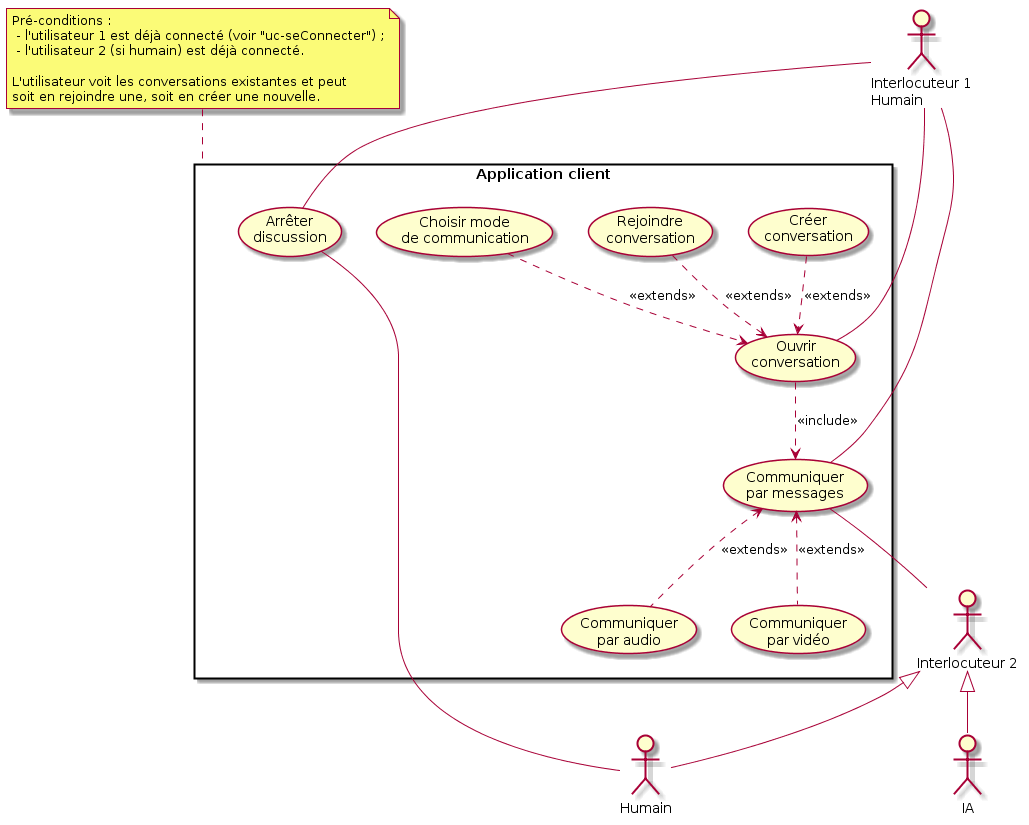
\includegraphics[scale=0.55]{images/uc-discuter.png}
%\caption{Cas d'utilisation \textbf{discuter}}
%\label{cas1}
%\end{figure}
%Le cas d'utilisation (figure \ref{cas1}) représente les interactions entre les différents interlocuteurs et les différents moyens mis à leur disposition pour communiquer.

%\begin{center}
%\begin{figure}[H]
%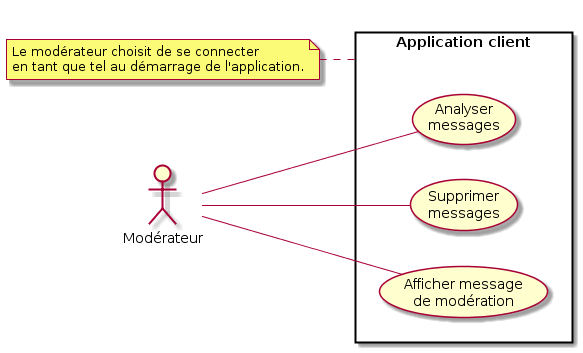
\includegraphics[scale=0.7]{images/uc-filtrerMessages.png}
%\vspace{5\baselineskip}
%\caption{Cas d'utilisation \textbf{filtrer les messages}}
%\end{figure}

%\begin{figure}
%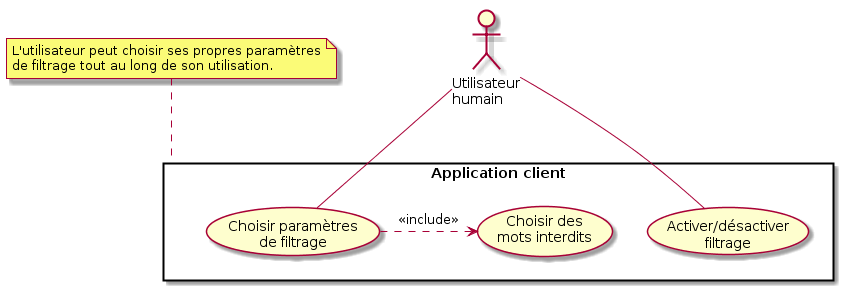
\includegraphics[scale=0.6]{images/uc-parametrerFiltrage.png}
%\caption{Cas d'utilisation \textbf{paramétrer le filtrage}}
%\end{figure}
%
%\begin{figure}
%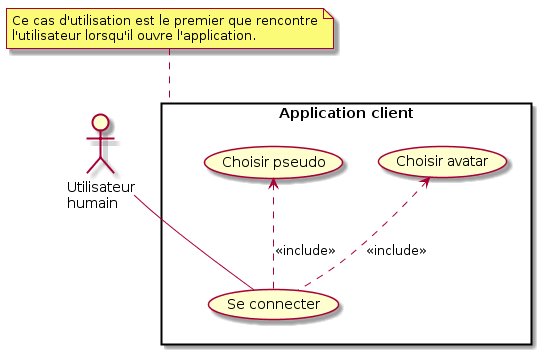
\includegraphics[scale=0.7]{images/uc-seConnecter.png}
%\caption{Cas d'utilisation \textbf{se connecter}}
%\end{figure}
%
%\end{center}

\section{Spécifications d'interfaces}
\subsection*{Maquettes}

Cette section présente les maquettes de l'application.

%\begin{figure}[H]
%\centerline{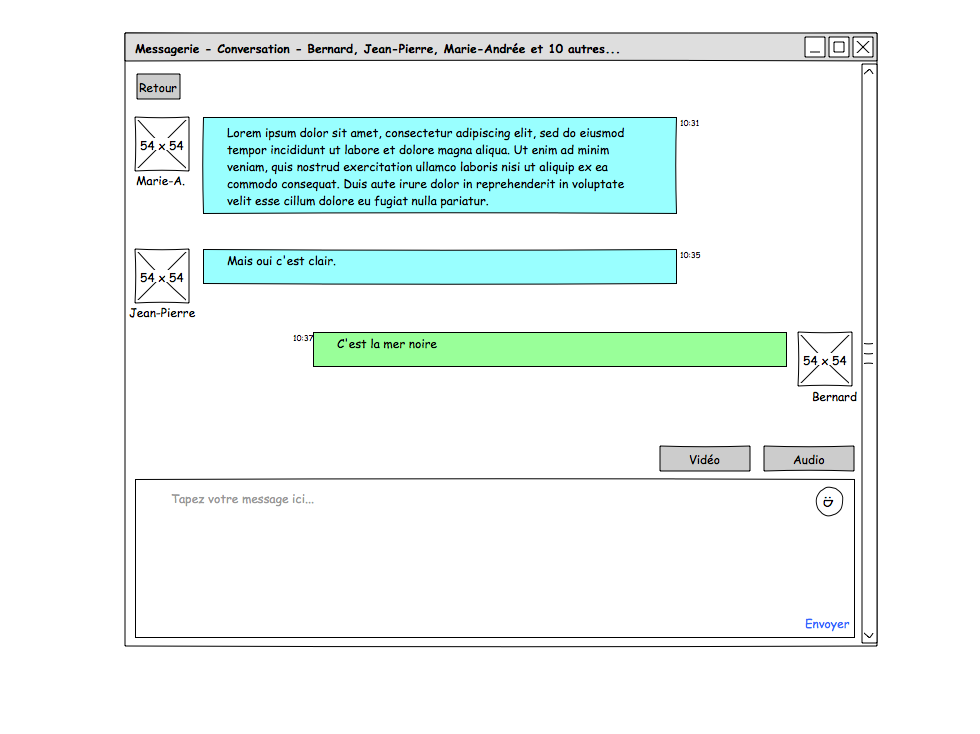
\includegraphics[width=0.95\textwidth]{maquette/maquette1.png}}
%\caption{Un exemple de conversation texte}
%\end{figure}
%
%\begin{figure}[H]
%\centerline{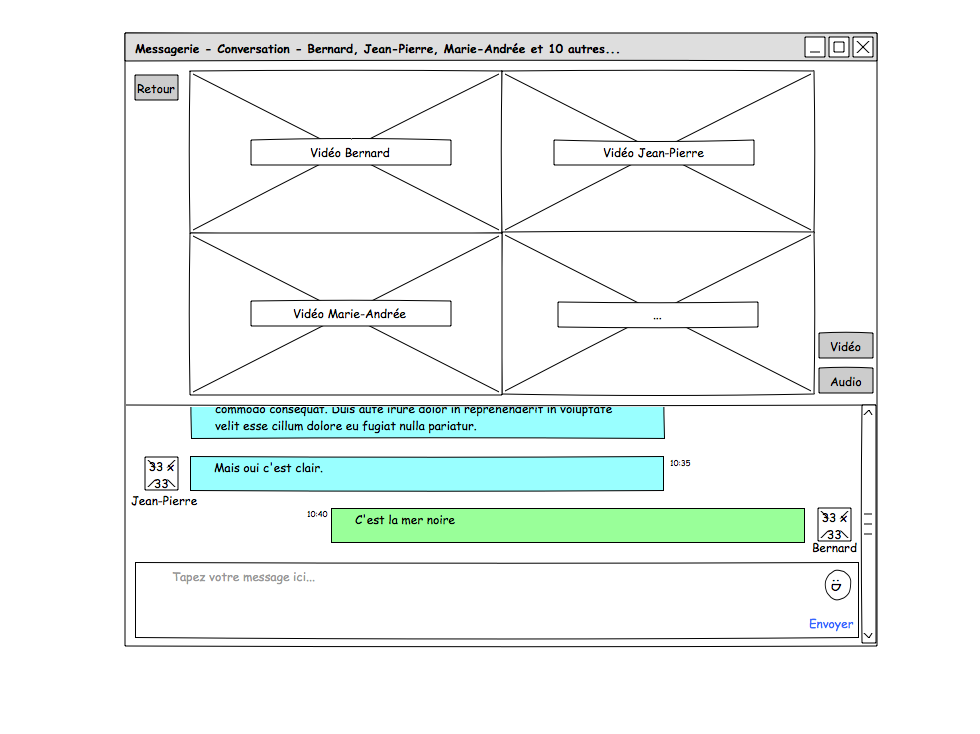
\includegraphics[width=0.9\textwidth]{maquette/maquette4.png}}
%\caption{Conversation vidéo}
%\end{figure}
%
%\begin{figure}[H]
%\centerline{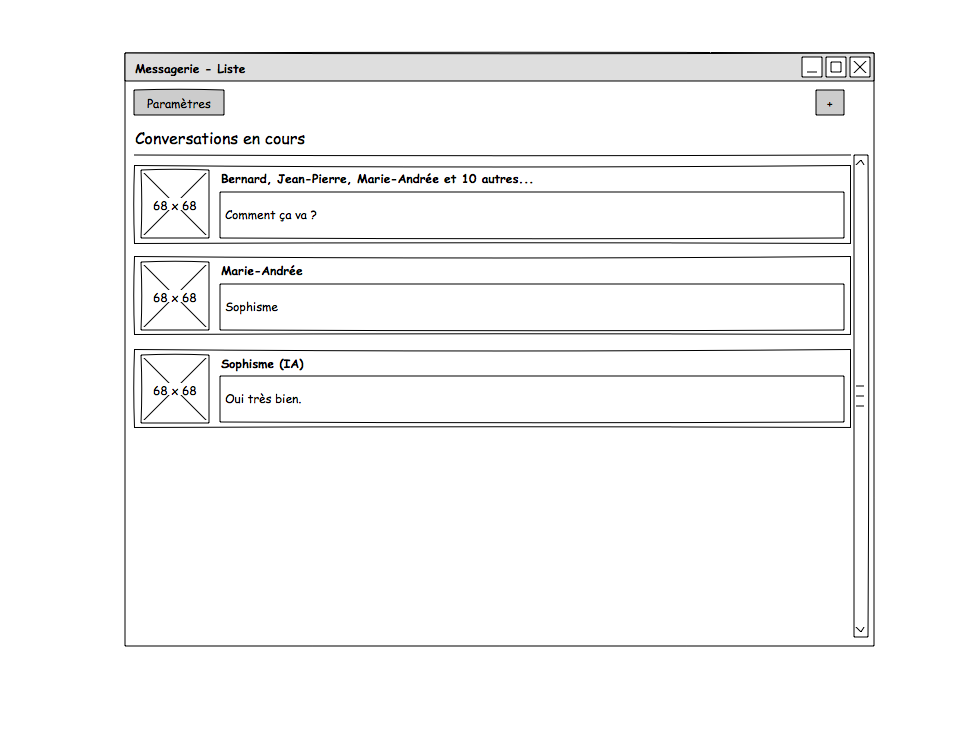
\includegraphics[width=0.9\textwidth]{maquette/maquette2.png}}
%\caption{Liste des conversations}
%\end{figure}
%
%\begin{figure}[H]
%\centerline{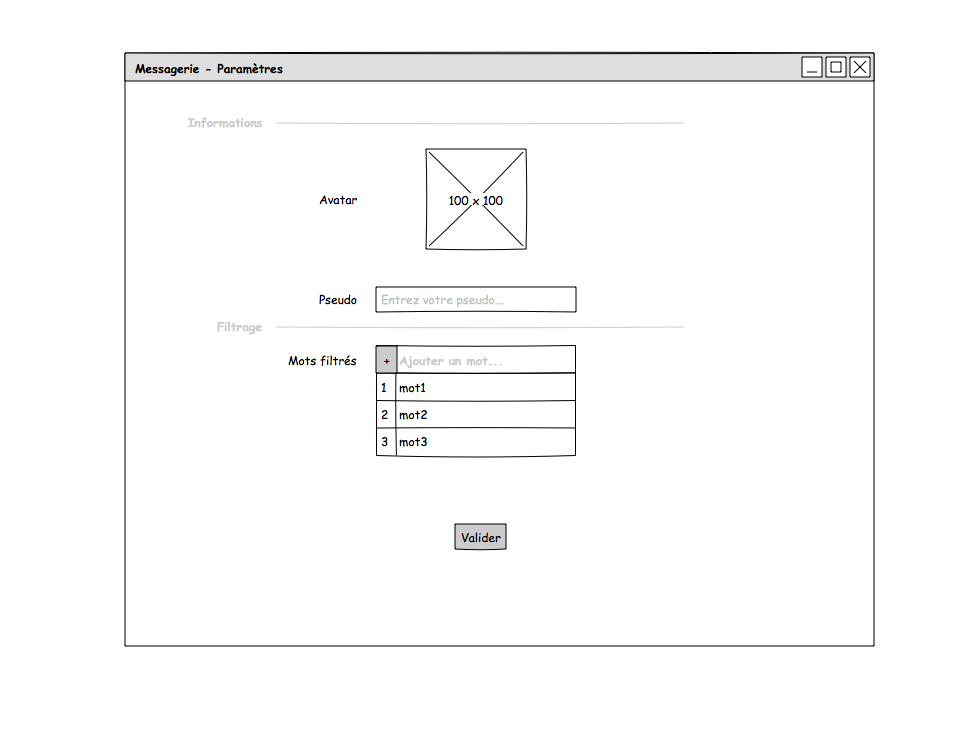
\includegraphics[width=0.9\textwidth]{maquette/maquette3.png}}
%\caption{Interface des paramètres}
%\end{figure}


\section{Spécifications opérationnelles}

Le système de messagerie répond instantanément.

De plus, les messages sont sauvegardés tant qu'il subsiste un utilisateur connecté à la conversation.

Le serveur qui héberge l'application est disponible à chaque instant $t$ pour permettre aux utilisateurs d'utiliser le service à n'importe quel moment.

Lors de l'utilisation de l'application, la reférence du compte est utilisée pour savoir qui participe à la conversation. Cette référence du compte transite donc entre l'application client et l'application serveur. Aucune mesure de sécurité n'est prévue pour éviter une transmission visible de cette référence.

\chapter{Conception préliminaire}

\section{Modèle du domaine}

%\begin{figure}[H]
%\centerline{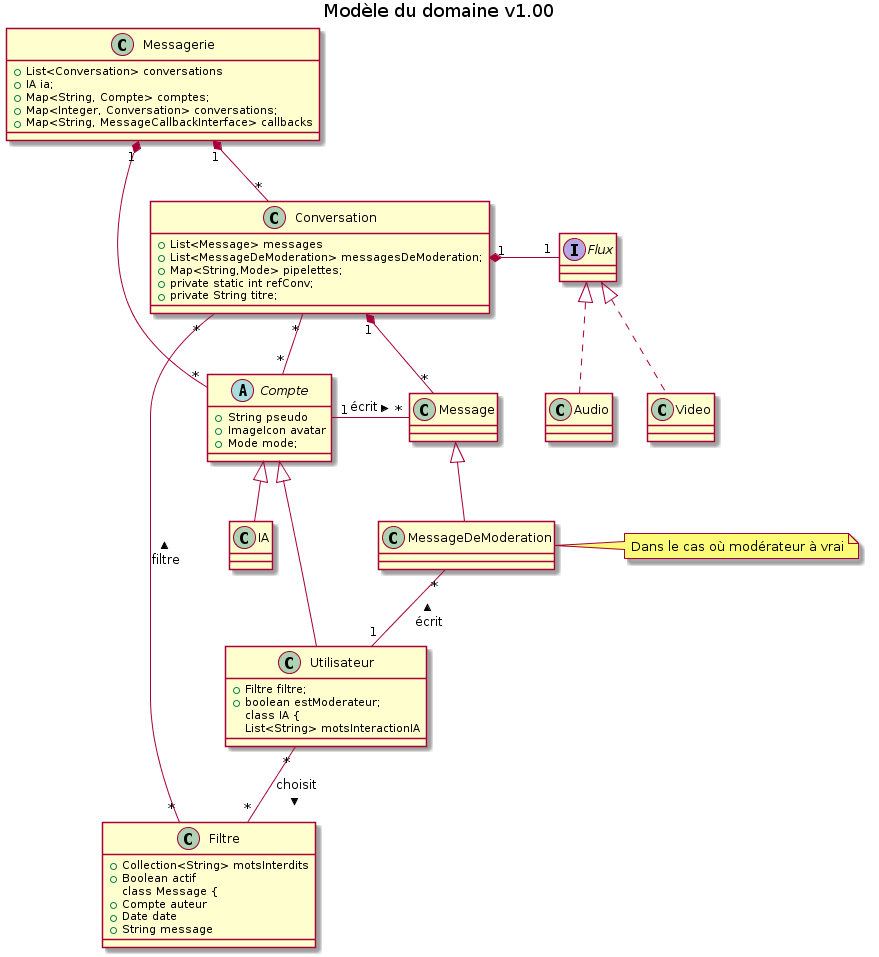
\includegraphics[width=0.95\textwidth]{diagrammes/class-diag.png}}
%\caption{Modèle du domaine}
%\end{figure}

\section{Diagrammes de séquence système}

%\begin{figure}[H]
%\centerline{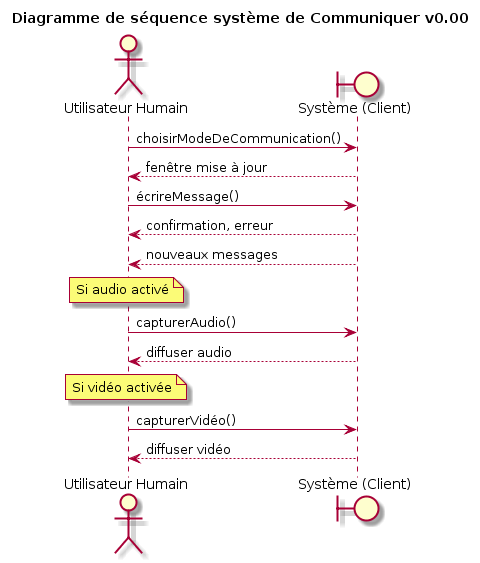
\includegraphics[width=0.9\textwidth]{diagrammes/dss-communiquer.png}}
%\caption{Le diagramme de séquence système de \og communiquer \fg}
%\end{figure}

%\begin{figure}[H]
%\centerline{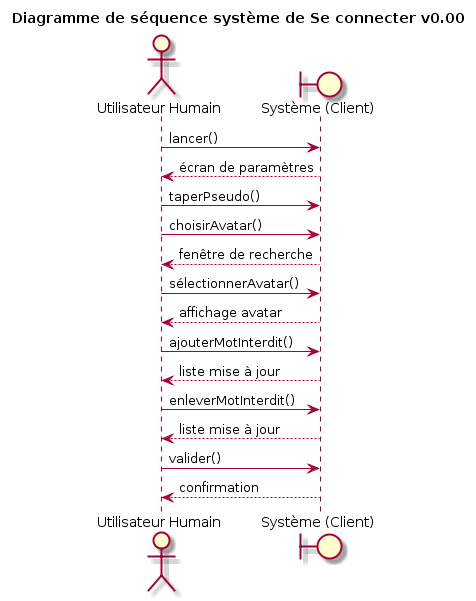
\includegraphics[width=0.9\textwidth]{diagrammes/dss-connexion.png}}
%\caption{Le diagramme de séquence système de \og se connecter \fg}
%\end{figure}

%\begin{figure}[H]
%\centerline{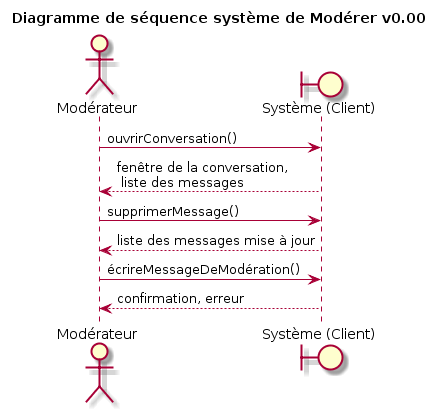
\includegraphics[width=0.9\textwidth]{diagrammes/dss-moderer.png}}
%\caption{Le diagramme de séquence système de \og modérer \fg}
%\end{figure}

\subsection{Modification du modèle du domaine}
La logique utilisée lors de la conception est restée la même. Nous avons cependant effectuée 2 changements principaux. Nous avons inclus beaucoup plus de champs dans la classe Messagerie. En effet nous avons tous centraliser via cette classe pour structurer les encapsulations. Par exemple, cette classe contient l'IA. \\
De plus, nous avions initialement une classe modérateur que nous avons supprimé et transformé en un booléen dans la classe utilisateur. Choix qui nous paraissait beaucoup plus pertinent.

\section{Diagrammes d'activités}
%\begin{figure}[H]
%\centerline{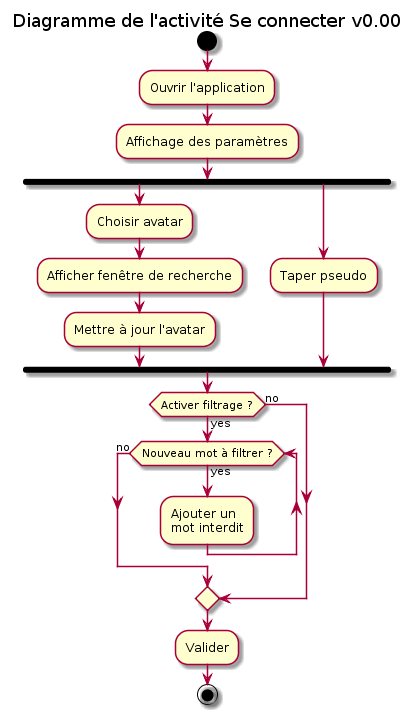
\includegraphics[width=0.75\textwidth]{diagrammes/activity-settings-diag.png}}
%\caption{Le diagramme de l'activité \og se connecter \fg}
%\end{figure}
%
%\begin{figure}[H]
%\centerline{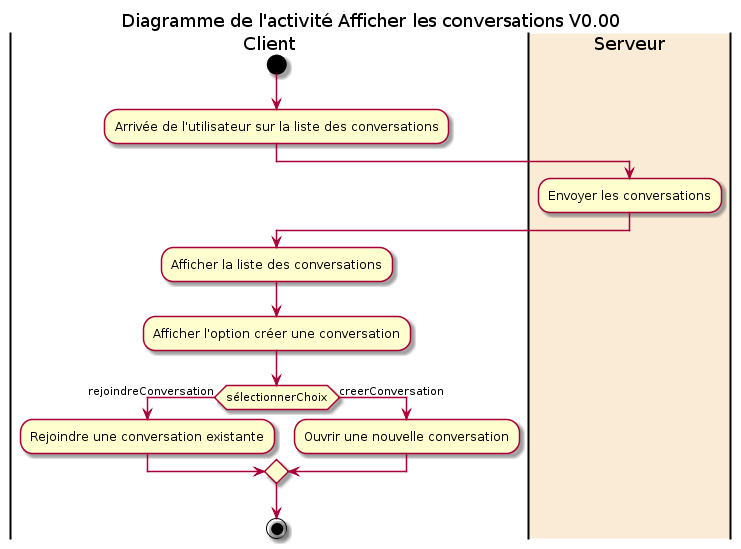
\includegraphics[width=0.95\textwidth]{diagrammes/activity-convList-diag.png}}
%\caption{Le diagramme de l'activité \og choisir une conversation \fg}
%\end{figure}
%
%\begin{figure}[H]
%\centerline{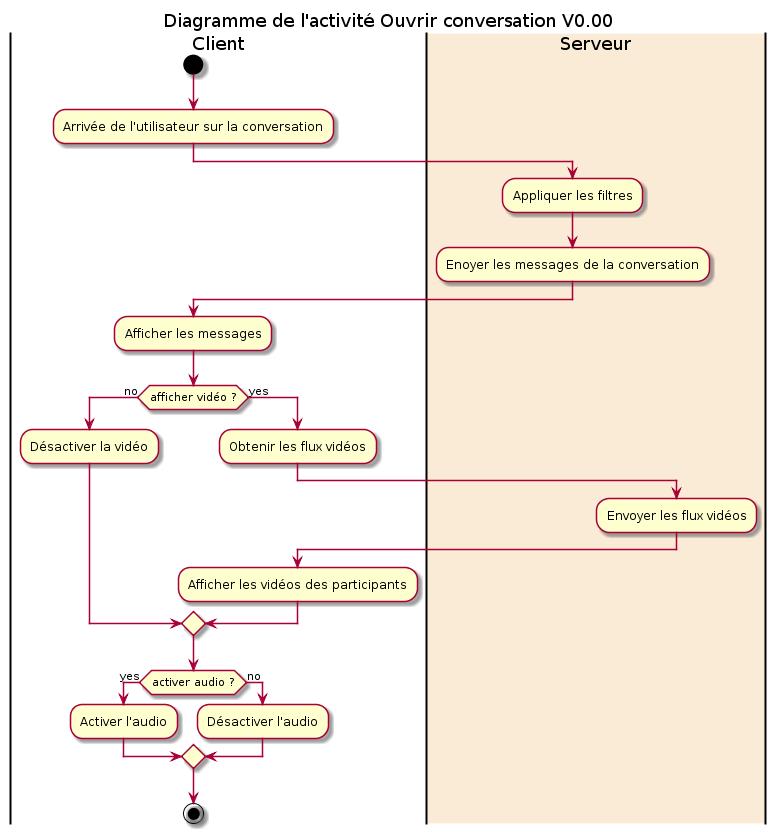
\includegraphics[width=0.75\textwidth]{diagrammes/activity-openConv-diag.png}}
%\caption{Le diagramme de l'activité \og ouvrir une conversation \fg}
%\end{figure}
%
%\begin{figure}[H]
%\centerline{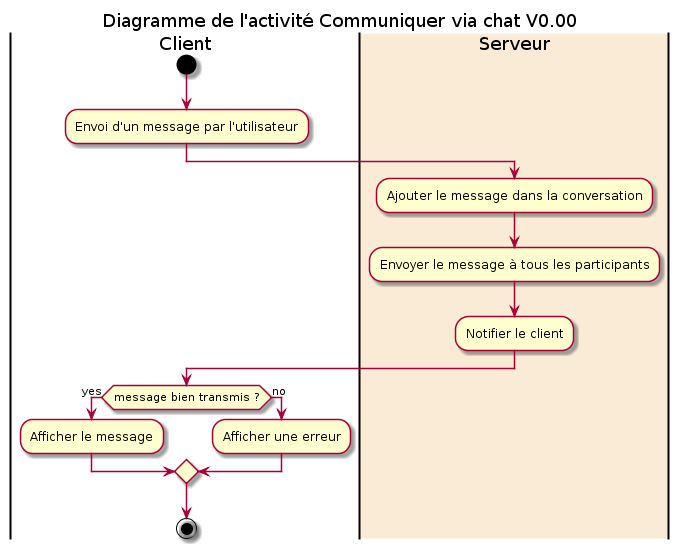
\includegraphics[width=0.8\textwidth]{diagrammes/activity-sendMsg-diag.png}}
%\caption{Le diagramme de l'activité \og communiquer \fg}
%\end{figure}


\section{Diagrammes d’interaction}

%\begin{figure}[H]
%\centerline{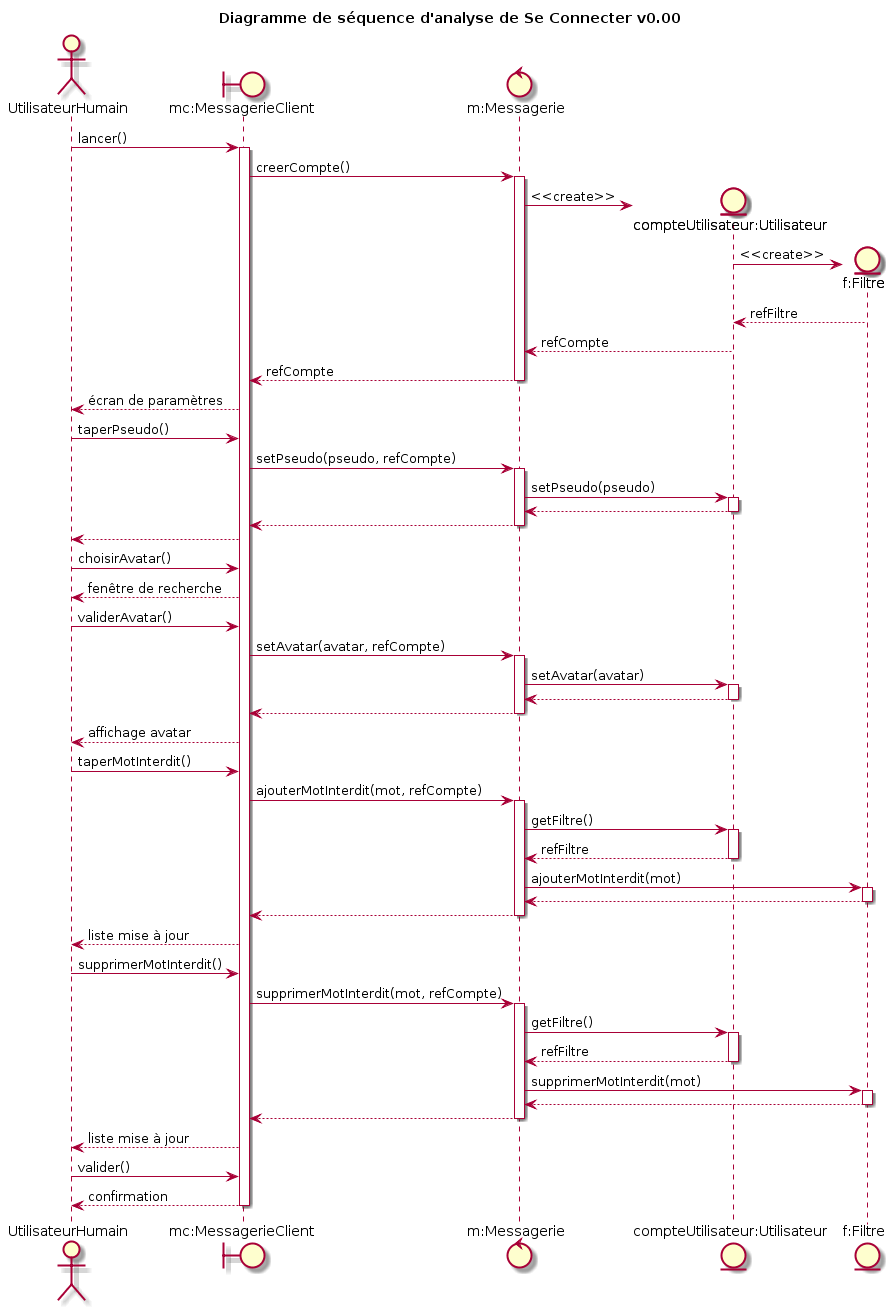
\includegraphics[width=0.9\textwidth]{diagrammes/dsa-connexion.png}}
%\caption{Le diagramme de séquence d'analyse \og se connecter \fg}
%\end{figure}
%
%\begin{figure}[H]
%\centerline{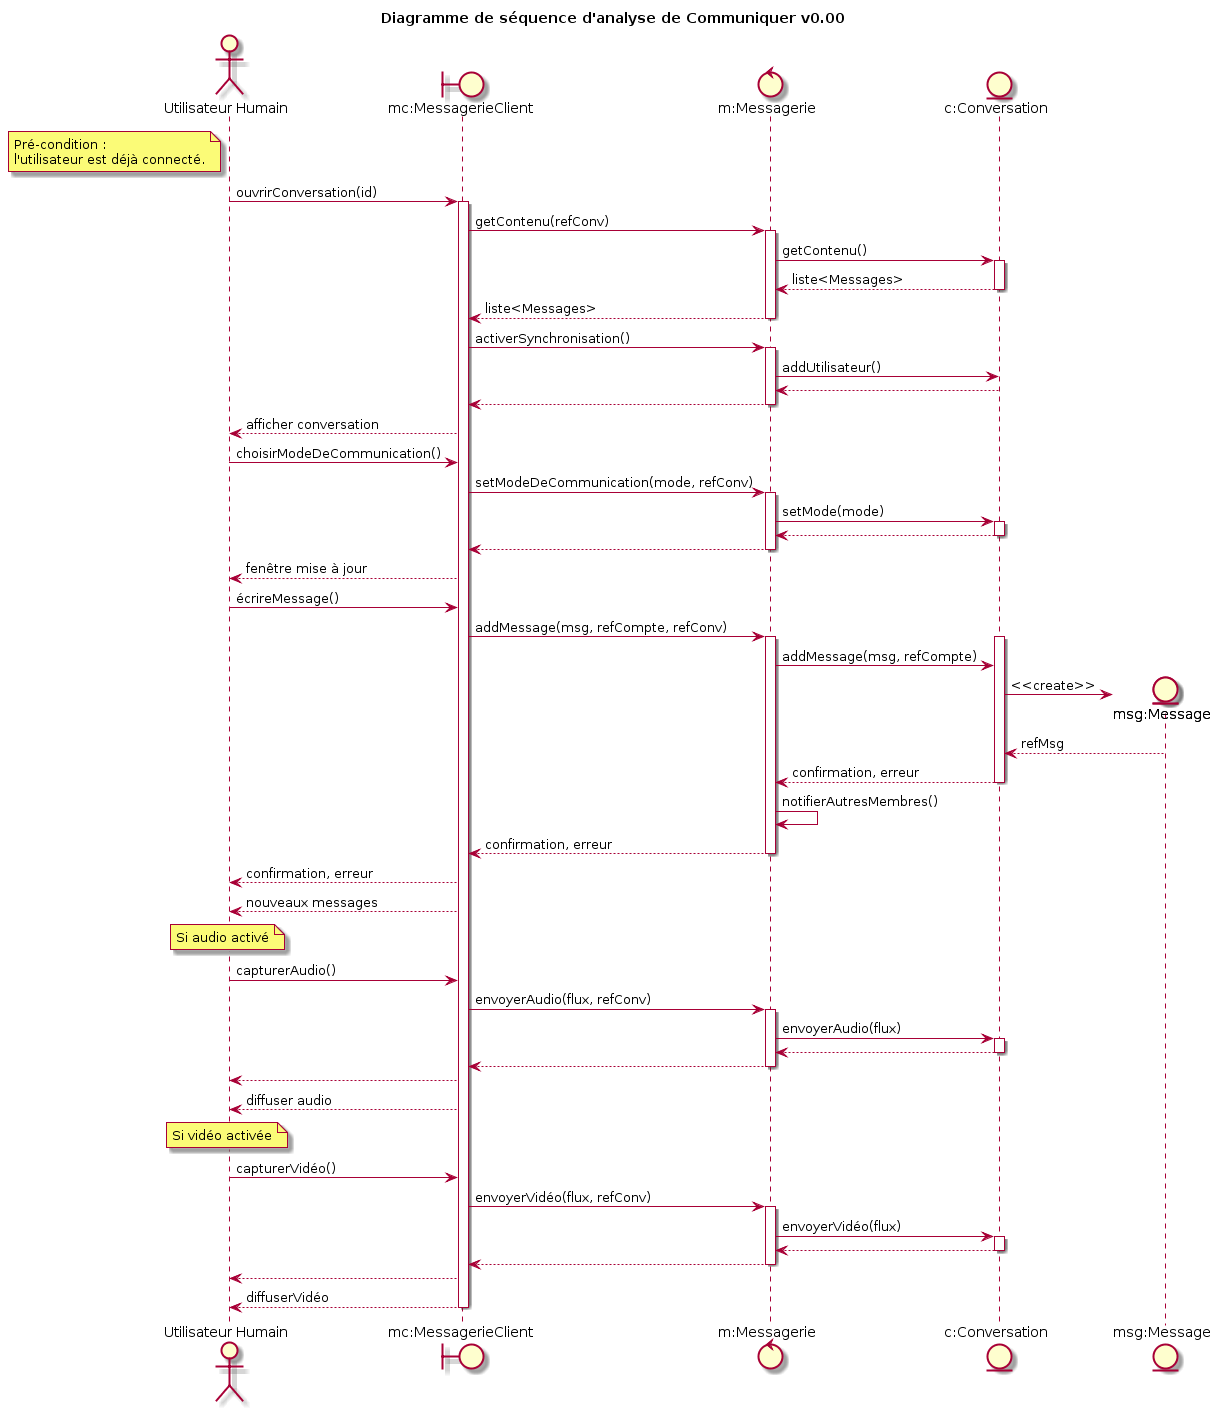
\includegraphics[width=0.9\textwidth]{diagrammes/dsa-communiquer.png}}
%\caption{Le diagramme de séquence d'analyse \og Communiquer \fg}
%\end{figure}
%
%\begin{figure}[H]
%\centerline{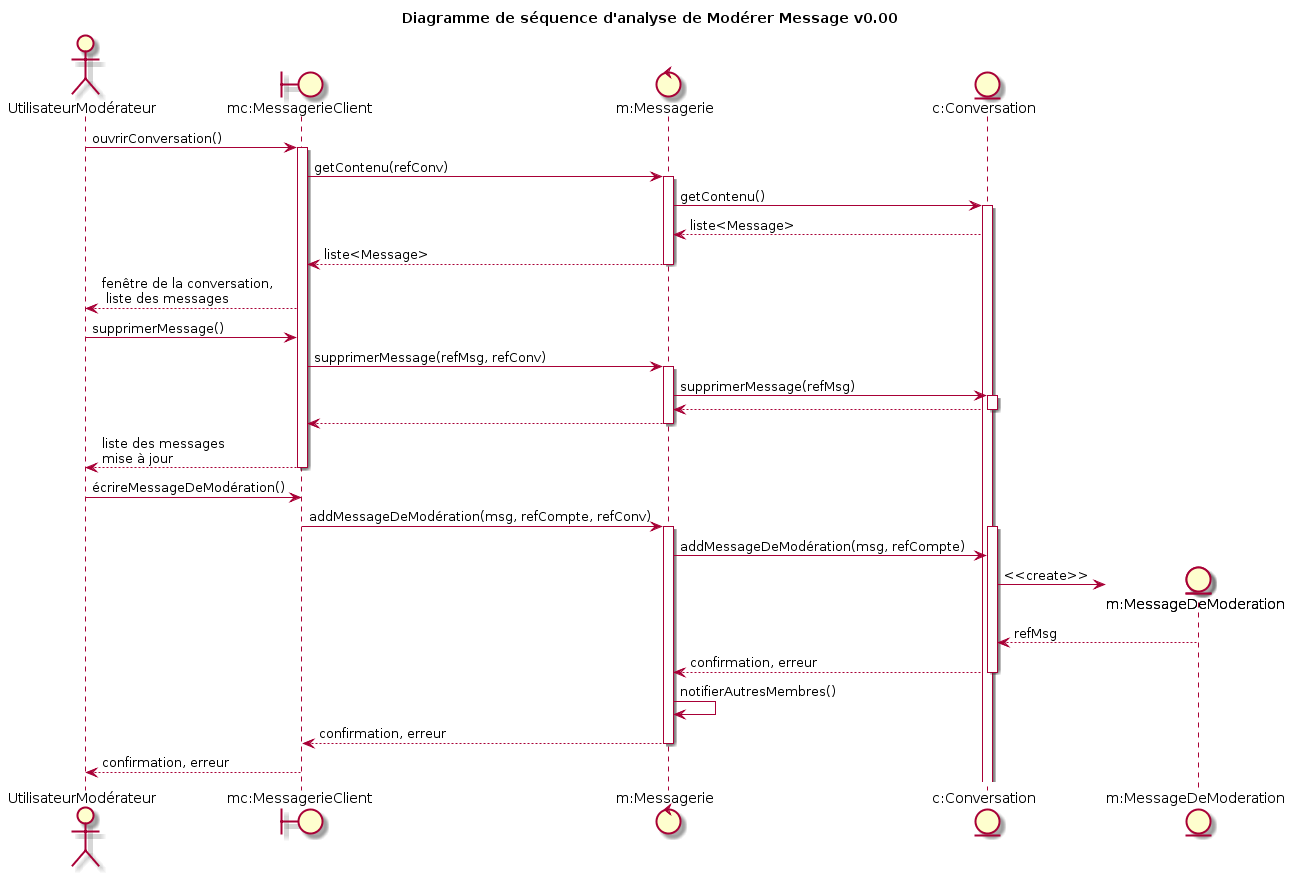
\includegraphics[width=0.75\textwidth]{diagrammes/dsa-moderer.png}}
%\caption{Le diagramme de séquence d'analyse \og Modérer Message \fg}
%\end{figure}

\section{Diagramme de communication client serveur}

\section{Découpage de l'application en \emph{packages}}
%\begin{figure}[H]
%\centerline{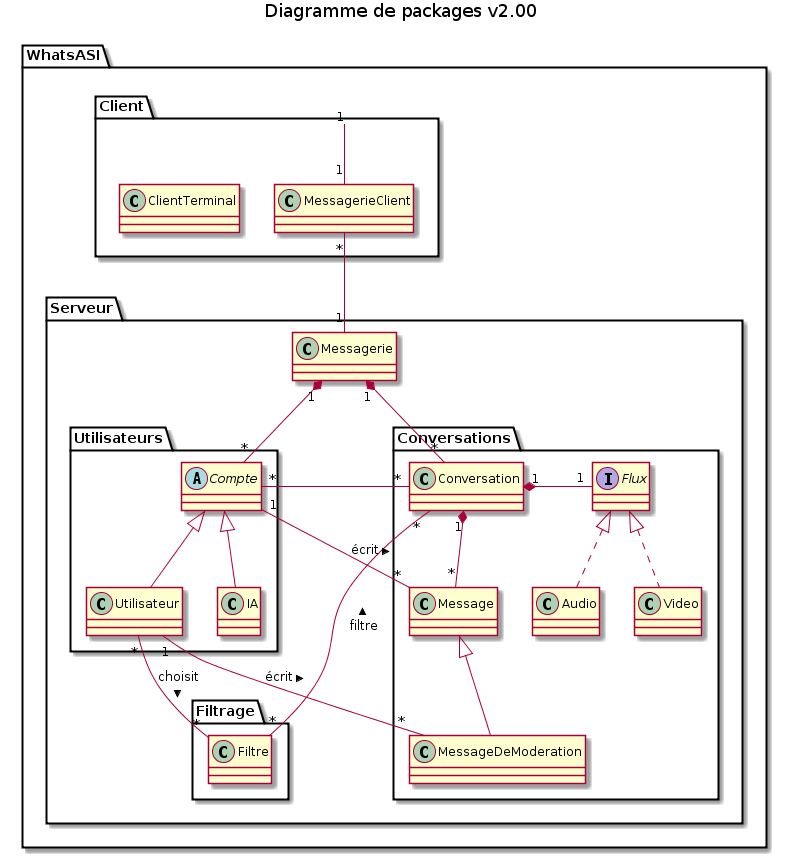
\includegraphics[width=0.8\textwidth]{diagrammes/package-diag.png}}
%\caption{Le diagramme de packages}
%\end{figure}


%\paragraph*{Classe Messagerie}
%\begin{itemize}
%\item \texttt{public List<Conversation> getConversations()} ;
%\end{itemize}
%
%\paragraph*{Classe Conversation}
%\begin{itemize}
%\item \texttt{public List<Message> getMessages()} ;
%\item \texttt{public List<Compte> getListeParticipants()} ;
%\item \texttt{public void afficherConversation()} ;
%\item \texttt{public void supprMessageInList(Message msg)} ;
%\item \texttt{public void broadcastInMsg()} ;
%\item \texttt{public void addMessageInList(Message msg)} ;
%
%\end{itemize}
%
%\paragraph*{Interface Video}
%\begin{itemize}
%\item \texttt{public void startVideo()} ;
%\item \texttt{public void endVideo()} ;
%\end{itemize}
%
%\paragraph*{Interface Audio}
%\begin{itemize}
%\item \texttt{public void startAudio()} ;
%\item \texttt{public void endAudio()} ;
%\end{itemize}
%
%\paragraph*{Classe Message}
%\begin{itemize}
%\item \texttt{public Compte getAuteur()} ;
%\item \texttt{public Date getDate()} ;
%\item \texttt{public String getMessage()} ;
%\end{itemize}
%
%\paragraph*{Classe MessageDeModeration}
%\begin{itemize}
%\item \texttt{public void sendMessageDeModeration(String message)} ;
%
%\end{itemize}
%
%\subsubsection{\og Gestion des utilisateurs \fg}
%
%\paragraph*{Classe Abstraite Compte}
%\begin{itemize}
%\item \texttt{public String getPseudo()} ;
%\item \texttt{public ImageIcon getAvatar()} ;
%\item \texttt{public boolean canVideo()} ;
%\item \texttt{public boolean canAudio()} ;
%\item \texttt{public void setVideo(boolean b)} ;
%\item \texttt{public void setAudio(boolean b)} ;
%\end{itemize}
%
%\paragraph*{Classe Moderateur}~\\
%Hérite de la classe abstraite \texttt{Compte}.
%\begin{itemize}
%\item \texttt{public void selectionnerConversation()} ;
%\item \texttt{public bool supprimerMessage(Message msg)} ;
%\item \texttt{public void messageDeModeration(Message msg)} ;
%\end{itemize}
%
%\paragraph*{Classe IA}~\\
%Hérite de la classe abstraite \texttt{Compte}.
%\begin{itemize}
%\item \texttt{public Collection<String> getMessagesPossiblesIA()} ;
%\item \texttt{public String answerMessage(String messageRecu)} ;
%\end{itemize}
%
%\paragraph*{Classe Utilisateur}~\\
%Hérite de la classe abstraite \texttt{Compte}.
%\begin{itemize}
%\item \texttt{public Filtre getFiltre()} ;
%\item \texttt{public void selectionModificationDeCompte()} ;
%\item \texttt{public void modifierAvatar()} ;
%\item \texttt{public void selectionImage()} ;
%\item \texttt{public void modifierPseudo()} ;
%\end{itemize}
%
%
%\subsubsection{\og Gestion du filtrage \fg}
%
%\paragraph*{Classe Filtre}
%\begin{itemize}
%\item \texttt{public Collection<String> getMotsInterdits()} ;
%\item \texttt{public void addMotInterdit(String mot)} ;
%\end{itemize}
%

Nous avons choisi de travailler avec des threads et callback. Comme indiqué sur la figure ci dessous. Nous sommes en multiclient: il y a donc un callback par client.



\chapter{Conception détaillée}
%\begin{figure}[H]
%\centerline{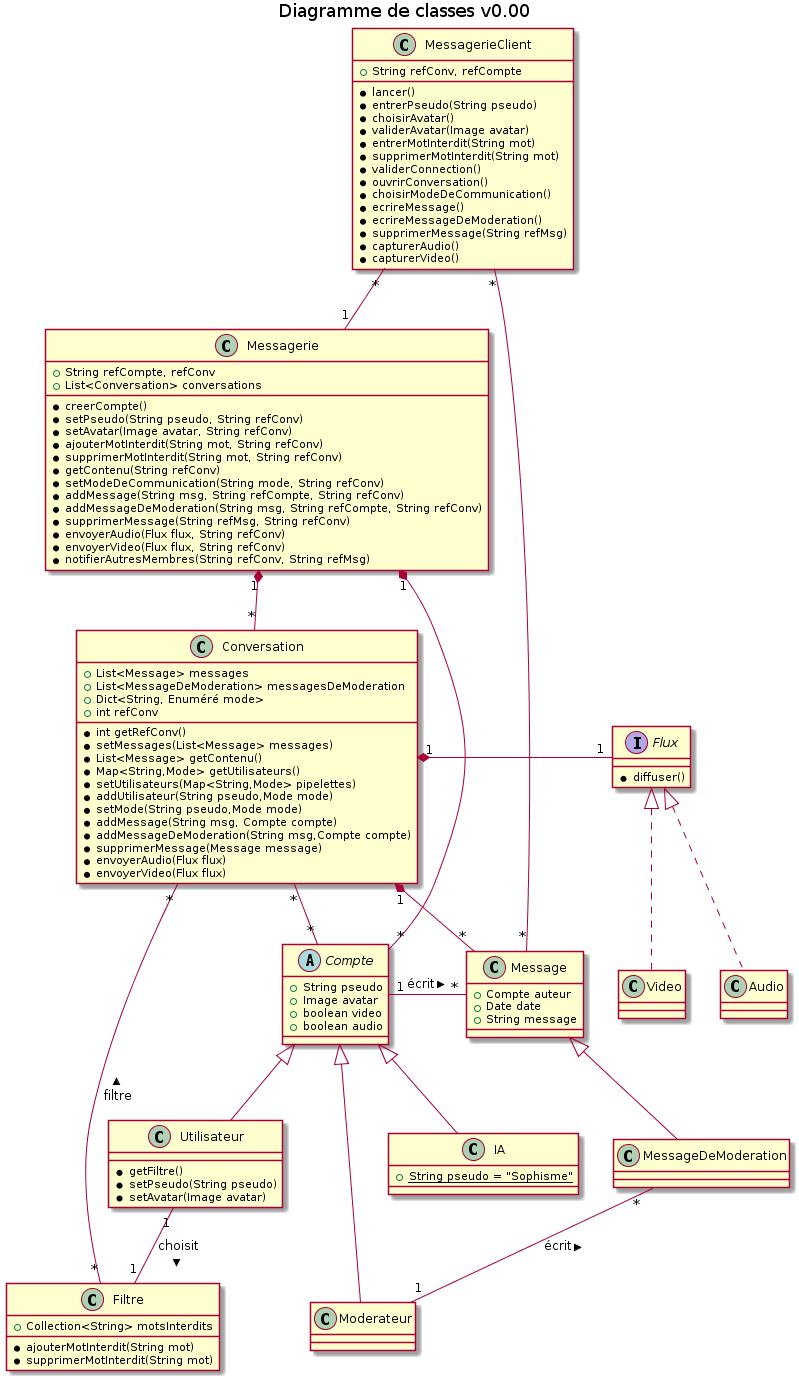
\includegraphics[width=0.7\textwidth]{diagrammes/detailedConception.png}}
%\caption{Le diagramme de classes de conception détaillée}
%\end{figure}
\chapter{Implémentations et tests}
L'objectif de cette partie est de préciser nos différents choix techniques. De même que de justifier le bon fonctionnement de nos fonctionnalités.
\section{Choix techniques}
\subsection{Langage de programmation, librairie, technologie pour la notion d'informatique répartie}
\subsubsection{Langage de programmation}
Nous avons choisi d'utiliser un langage orienté objet : JAVA. L'utilisation d'un tel langage nous paraissait pertinente et adaptée à notre projet que nous voulions orienté logiciel.\\
Premièrement, il était assez simple de passer d'une conception UML à une programmation JAVA. \\
Deuxièmement JAVA permettait la gestion des exceptions.\\
De plus ce langage est celui le plus maîtrisé par l'ensemble du groupe.
Enfin il s'adaptait parfaitement à l'utilisation de RMI.\\
\subsubsection{Librairie}
Nous avons choisi d'utiliser java-fx, qui offre un certain nombre de fonctionnalités graphiques. Cela nous permettait de découvrir une nouvelle librairie sachant que nous connaissions déjà swing.
\subsubsection{Technologie pour la notion d'informatique répartie}
Nous avons fait le choix d'utiliser un système de communication RMI avec de l'appel de méthode sur des objets distants. Nous avons choisi cette technologie car elle n'est pas orientée WEB de façon pure (moins que REST) et nous souhaitions réaliser un travail basé sur un logiciel et non un site WEB.\\
De plus il était nécessaire d'utiliser des threads pour avoir plusieurs clients. 
\subsection{Guide d'utilisation}
Voici les différentes étapes à suivre pour utiliser notre application:
\subsubsection{Concernant l'installation}
\begin{itemize}
\item Compiler le projet via le fichier compile.shs
\item Lancer le RmiRegistry ./launchRmiregistry.sh
\item Lancer le serveur ./launchServer.sh (terminal si version terminale)
\item Lancer le client dans un autre terminal ./launchClient.sh (terminal si version terminale)
\end{itemize}

\subsubsection{Concernant l'utilisation}
\begin{itemize}
\item Suivre les instructions présentes sur l'IHM
\item Pour lancer l'IA mettre \textbackslash bonjour, toutes les instructions apparaîtront.
\item compléter certains trucs
\end{itemize}

\section{Tests de validation}
A COMPLETER
\subsection{Tests des spécifications fonctionnelles}
\subsection{Tests des spécifications d'interface}
\subsection{Tests des spécifications opérationnelles}

\chapter{Conclusion et perspectives}
\section{Développement}
\subsection{Ce que nous avons développé}
\subsection{Ce que nous avons abandonné}
Nous n'avons pas pris le temps de réaliser l'échange via le flux audio et le flux vidéo par manque de temps.
\section{Ce qui aurait pu être ajouté}
Nous aurions pu ajouter une fonctionnalité qui permet de sécuriser le passage de la refconf.
\end{document}
